% !TEX TS-program = pdflatexmk
\documentclass[12pt]{article}

% Layout.
\usepackage[top=1in, bottom=0.75in, left=1in, right=1in, headheight=1in, headsep=6pt]{geometry}

% Fonts.
\usepackage{mathptmx}
\usepackage[scaled=0.86]{helvet}
\renewcommand{\emph}[1]{\textsf{\textbf{#1}}}
\newcommand{\ans}[1][1in]{\rule{#1}{.5pt}}

\usepackage[parfill]{parskip}

% Misc packages.
\usepackage{amsmath,amssymb,latexsym}
\usepackage{graphicx,hyperref}
\usepackage{array}
\usepackage{xcolor}
\usepackage{multicol,tikz}
\usepackage{tabularx,colortbl,booktabs,xparse}
\usepackage{enumitem}
\usetikzlibrary{calc}
\newcommand{\be}{\begin{enumerate}}
\newcommand{\ee}{\end{enumerate}}

% Rotation: \rot[<angle>][<width>]{<stuff>}
\NewDocumentCommand{\rot}{O{45} O{1em} m}{\makebox[#2][l]{\rotatebox{#1}{#3}}}%

\usepackage{fancyhdr}
\pagestyle{fancy} 
\lhead{\large\sf\textbf{MATH F113X: Three Hamiltonian Circuit Algorithms}}
%\chead{\large\sf\textbf{lecture notes}}
%\rhead{\large\sf\textbf{Day 1}}

\begin{document}
Two Distinct Questions\\

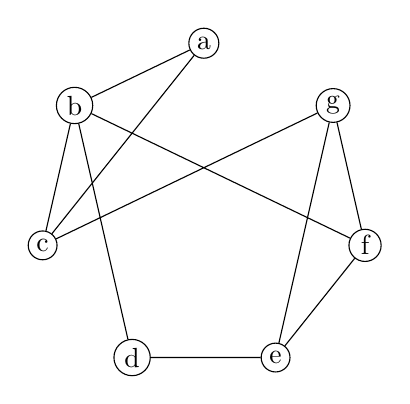
\begin{tikzpicture}[vtx/.style={draw, circle, inner sep =1.5 pt}, lbl/.style =  {inner sep =1.5 pt, fill = white}, scale = 0.7]
\foreach \i/\l in {0/a,1/b,2/c,3/d,4/e,5/f,6/g}{\node[vtx] (\i) at (360*\i/7+90:3){\l};}
\draw (0)-- (1)--(2) -- (0) (3) -- (1) -- (5) -- (6) -- (2)(3)--(4)--(5)(4)--(6);
\end{tikzpicture}
\hfill
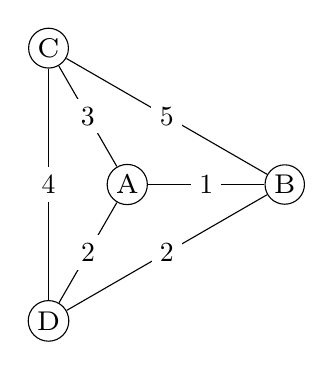
\begin{tikzpicture}[vtx/.style = {scale=1.4, draw, circle, inner sep = 1 pt,font = \scriptsize},
lbl/.style = {, fill = white, inner sep =3 pt}, scale = 1
]
\node[vtx] (A) at (0,0) {A};
\node[vtx] (B) at (0:2) {B};
\node[vtx] (C) at (120:2) {C};
\node[vtx] (D) at (240:2) {D};
\foreach \i/\j/\k in {A/B/1, A/C/3, A/D/2, B/C/5, B/D/2, C/D/4}{\draw (\i) --node[lbl, midway]{\k} (\j);}
\end{tikzpicture}

\vfill

\fbox{Brute Force Algorithm} \\

\vfill

\quad \hfill 
\fbox{
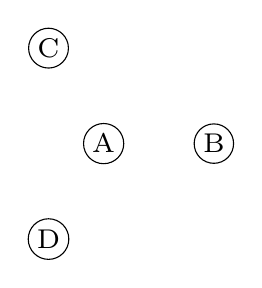
\begin{tikzpicture}[vtx/.style = {scale=1.4, draw, circle, inner sep = 1 pt,font = \scriptsize},
lbl/.style = {, fill = white, inner sep =3 pt}, scale = 0.7
]
\node[vtx] (A) at (0,0) {A};
\node[vtx] (B) at (0:2) {B};
\node[vtx] (C) at (120:2) {C};
\node[vtx] (D) at (240:2) {D};
\end{tikzpicture}
}
\quad \hfill 
\fbox{
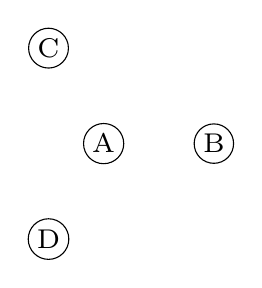
\begin{tikzpicture}[vtx/.style = {scale=1.4, draw, circle, inner sep = 1 pt,font = \scriptsize},
lbl/.style = {, fill = white, inner sep =3 pt}, scale = 0.7
]
\node[vtx] (A) at (0,0) {A};
\node[vtx] (B) at (0:2) {B};
\node[vtx] (C) at (120:2) {C};
\node[vtx] (D) at (240:2) {D};
\end{tikzpicture}
}
\quad \hfill 
\fbox{
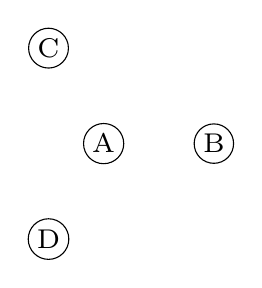
\begin{tikzpicture}[vtx/.style = {scale=1.4, draw, circle, inner sep = 1 pt,font = \scriptsize},
lbl/.style = {, fill = white, inner sep =3 pt}, scale = 0.7
]
\node[vtx] (A) at (0,0) {A};
\node[vtx] (B) at (0:2) {B};
\node[vtx] (C) at (120:2) {C};
\node[vtx] (D) at (240:2) {D};
\end{tikzpicture}
}



\quad \hfill 
\fbox{
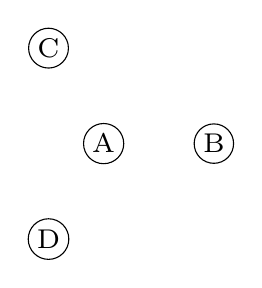
\begin{tikzpicture}[vtx/.style = {scale=1.4, draw, circle, inner sep = 1 pt,font = \scriptsize},
lbl/.style = {, fill = white, inner sep =3 pt}, scale = 0.7
]
\node[vtx] (A) at (0,0) {A};
\node[vtx] (B) at (0:2) {B};
\node[vtx] (C) at (120:2) {C};
\node[vtx] (D) at (240:2) {D};
\end{tikzpicture}
}
\quad \hfill 
\fbox{
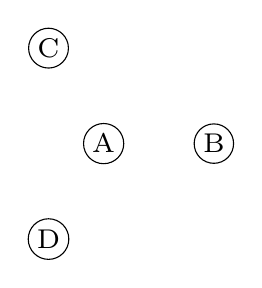
\begin{tikzpicture}[vtx/.style = {scale=1.4, draw, circle, inner sep = 1 pt,font = \scriptsize},
lbl/.style = {, fill = white, inner sep =3 pt}, scale = 0.7
]
\node[vtx] (A) at (0,0) {A};
\node[vtx] (B) at (0:2) {B};
\node[vtx] (C) at (120:2) {C};
\node[vtx] (D) at (240:2) {D};
\end{tikzpicture}
}
\quad \hfill
\fbox{
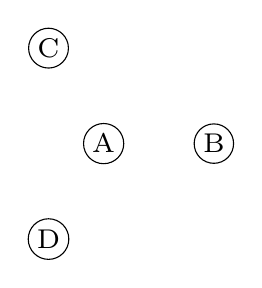
\begin{tikzpicture}[vtx/.style = {scale=1.4, draw, circle, inner sep = 1 pt,font = \scriptsize},
lbl/.style = {, fill = white, inner sep =3 pt}, scale = 0.7
]
\node[vtx] (A) at (0,0) {A};
\node[vtx] (B) at (0:2) {B};
\node[vtx] (C) at (120:2) {C};
\node[vtx] (D) at (240:2) {D};
\end{tikzpicture}
}

\newpage
\fbox{Nearest Neighbor Algorithm (NNA)} 
\vspace{1in}
 
 
 On the graph below, complete nearest neighbor starting with starting vertex A. What happens if you start at B?
 
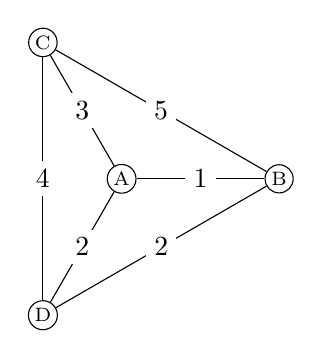
\begin{tikzpicture}[vtx/.style = {draw, circle, inner sep = 1 pt, font = \scriptsize},
lbl/.style = {, fill = white, inner sep =3 pt}
]
\node[vtx] (A) at (0,0) {A};
\node[vtx] (B) at (0:2) {B};
\node[vtx] (C) at (120:2) {C};
\node[vtx] (D) at (240:2) {D};
%\node[vtx] (E) at (240:2) {E};
\foreach \i/\j/\k in {A/B/1, A/C/3, A/D/2, B/C/5, B/D/2, C/D/4}{\draw (\i) --node[lbl, midway]{\k} (\j);}
\end{tikzpicture}
\hspace{1in}
\fbox{\\
\quad
\begin{tikzpicture}[vtx/.style = {draw, circle, inner sep = 1 pt, font = \scriptsize},
lbl/.style = {, fill = white, inner sep =3 pt}
]
\node[vtx] (A) at (0,0) {A};
\node[vtx] (B) at (0:2) {B};
\node[vtx] (C) at (120:2) {C};
\node[vtx] (D) at (240:2) {D};
\end{tikzpicture}}
\hspace{1in}
\fbox{\\
\quad
\begin{tikzpicture}[vtx/.style = {draw, circle, inner sep = 1 pt, font = \scriptsize},
lbl/.style = {, fill = white, inner sep =3 pt}
]
\node[vtx] (A) at (0,0) {A};
\node[vtx] (B) at (0:2) {B};
\node[vtx] (C) at (120:2) {C};
\node[vtx] (D) at (240:2) {D};
\end{tikzpicture}}

\fbox{Repeated Nearest Neighbor Algorithm (RNNA)} 
\vfill
On the graph below, complete the Repeated Nearest Neighbor.
 
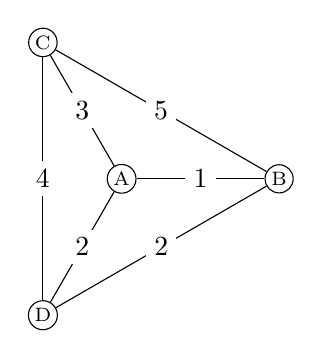
\begin{tikzpicture}[vtx/.style = {draw, circle, inner sep = 1 pt, font = \scriptsize},
lbl/.style = {, fill = white, inner sep =3 pt}
]
\node[vtx] (A) at (0,0) {A};
\node[vtx] (B) at (0:2) {B};
\node[vtx] (C) at (120:2) {C};
\node[vtx] (D) at (240:2) {D};
%\node[vtx] (E) at (240:2) {E};
\foreach \i/\j/\k in {A/B/1, A/C/3, A/D/2, B/C/5, B/D/2, C/D/4}{\draw (\i) --node[lbl, midway]{\k} (\j);}
\end{tikzpicture}
\hfill
\fbox{\\
\quad
\begin{tikzpicture}[vtx/.style = {draw, circle, inner sep = 1 pt, font = \scriptsize},
lbl/.style = {, fill = white, inner sep =3 pt}
]
\node[vtx] (A) at (0,0) {A};
\node[vtx] (B) at (0:2) {B};
\node[vtx] (C) at (120:2) {C};
\node[vtx] (D) at (240:2) {D};
\end{tikzpicture} \quad}
\hfill
\fbox{\\
\quad
\begin{tikzpicture}[vtx/.style = {draw, circle, inner sep = 1 pt, font = \scriptsize},
lbl/.style = {, fill = white, inner sep =3 pt}
]
\node[vtx] (A) at (0,0) {A};
\node[vtx] (B) at (0:2) {B};
\node[vtx] (C) at (120:2) {C};
\node[vtx] (D) at (240:2) {D};
\end{tikzpicture}\quad}



\newpage
Complete Repeated Nearest Neighbor on the graph below. (Suggestion: Use parallel processing)\\

\newcommand{\pic}{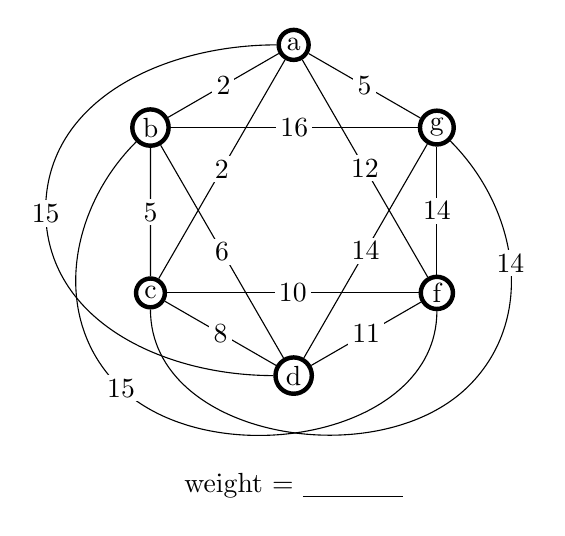
\begin{tikzpicture}[vtx/.style={draw, circle, inner sep =1.5 pt, ultra thick}, lbl/.style =  {inner sep =1.5 pt, fill = white, }, scale = .7]
\foreach \i/\l in {0/a,1/b,2/c,3/d,4/f,5/g}{\node[vtx] (\i) at (360*\i/6+90:3){\l};}
\draw (0) to [out=180,in=90] (180:4.5) to [out=270, in=180] node[lbl, pos = .01]{15} (3);
\draw (1) to [out=225,in=135] (225:4.5) to [out=315, in=270] node[lbl, pos = .01]{15} (4);
\draw (2) to [out=270,in=225] (315:4.5) to [out=45, in=315]  node[lbl, midway]{14}(5);
\foreach \i/\j/\k in {0/1/2, 0/2/2, 0/4/12, 0/5/5, 1/2/5, 1/3/6, 2/3/8, 2/4/10, 3/4/11, 3/5/14, 4/5/14, 1/5/16}{\draw (\i) -- node[lbl]{\k} (\j);}
\node at (0,-5){weight = \underline{\hspace{0.5in}}};
\end{tikzpicture}
}

\hfill \pic \hfill \pic \hfill

\hfill \pic \hfill \pic \hfill 

\hfill \pic \hfill \pic \hfill

\vfill
\Large{Conclusion:} 
\end{document}
